% ==============================================================================
%                                    DVG303
%                  Objektorienterad Design och Programmering
%                                Laboration #1
%
% Author:   Jonas Sjöberg
%           Högskolan i Gävle
%           tel12jsg@student.hig.se
%           https://github.com/jonasjberg
%
% License:  Creative Commons Attribution-NonCommercial-ShareAlike 4.0
%           International.  See LICENSE.md for full licensing information.
% ==============================================================================

\section*{Introduktion}\label{sec:intro}
\addcontentsline{toc}{section}{Introduktion}

\subsection*{Övergripande beskrivning}\label{sec:beskrivning}
\addcontentsline{toc}{subsection}{Övergripande beskrivning}
Det här är den första av tre laborationer i objektorienterad design och
programmering. Ett fullständigt program kommer att utvecklas under
laborationerna. Processen kommer att innehålla många element av professionell
mjukvaruutveckling; design, dokumentation, revisionskontroll, etc., och syftar
till att utveckla praktiska färdigheter i mjukvaruutveckling.

\subsection*{Specifikation}
\addcontentsline{toc}{subsection}{Specifikation}
Den funktionalitet som efterfrågas beskrivs enligt UML-standardiserat
användningsfallsdiagram (\emph{``use case diagram''}) i Figur~\ref{fig:usecase}.

\begin{figure}[htbp]
\centering
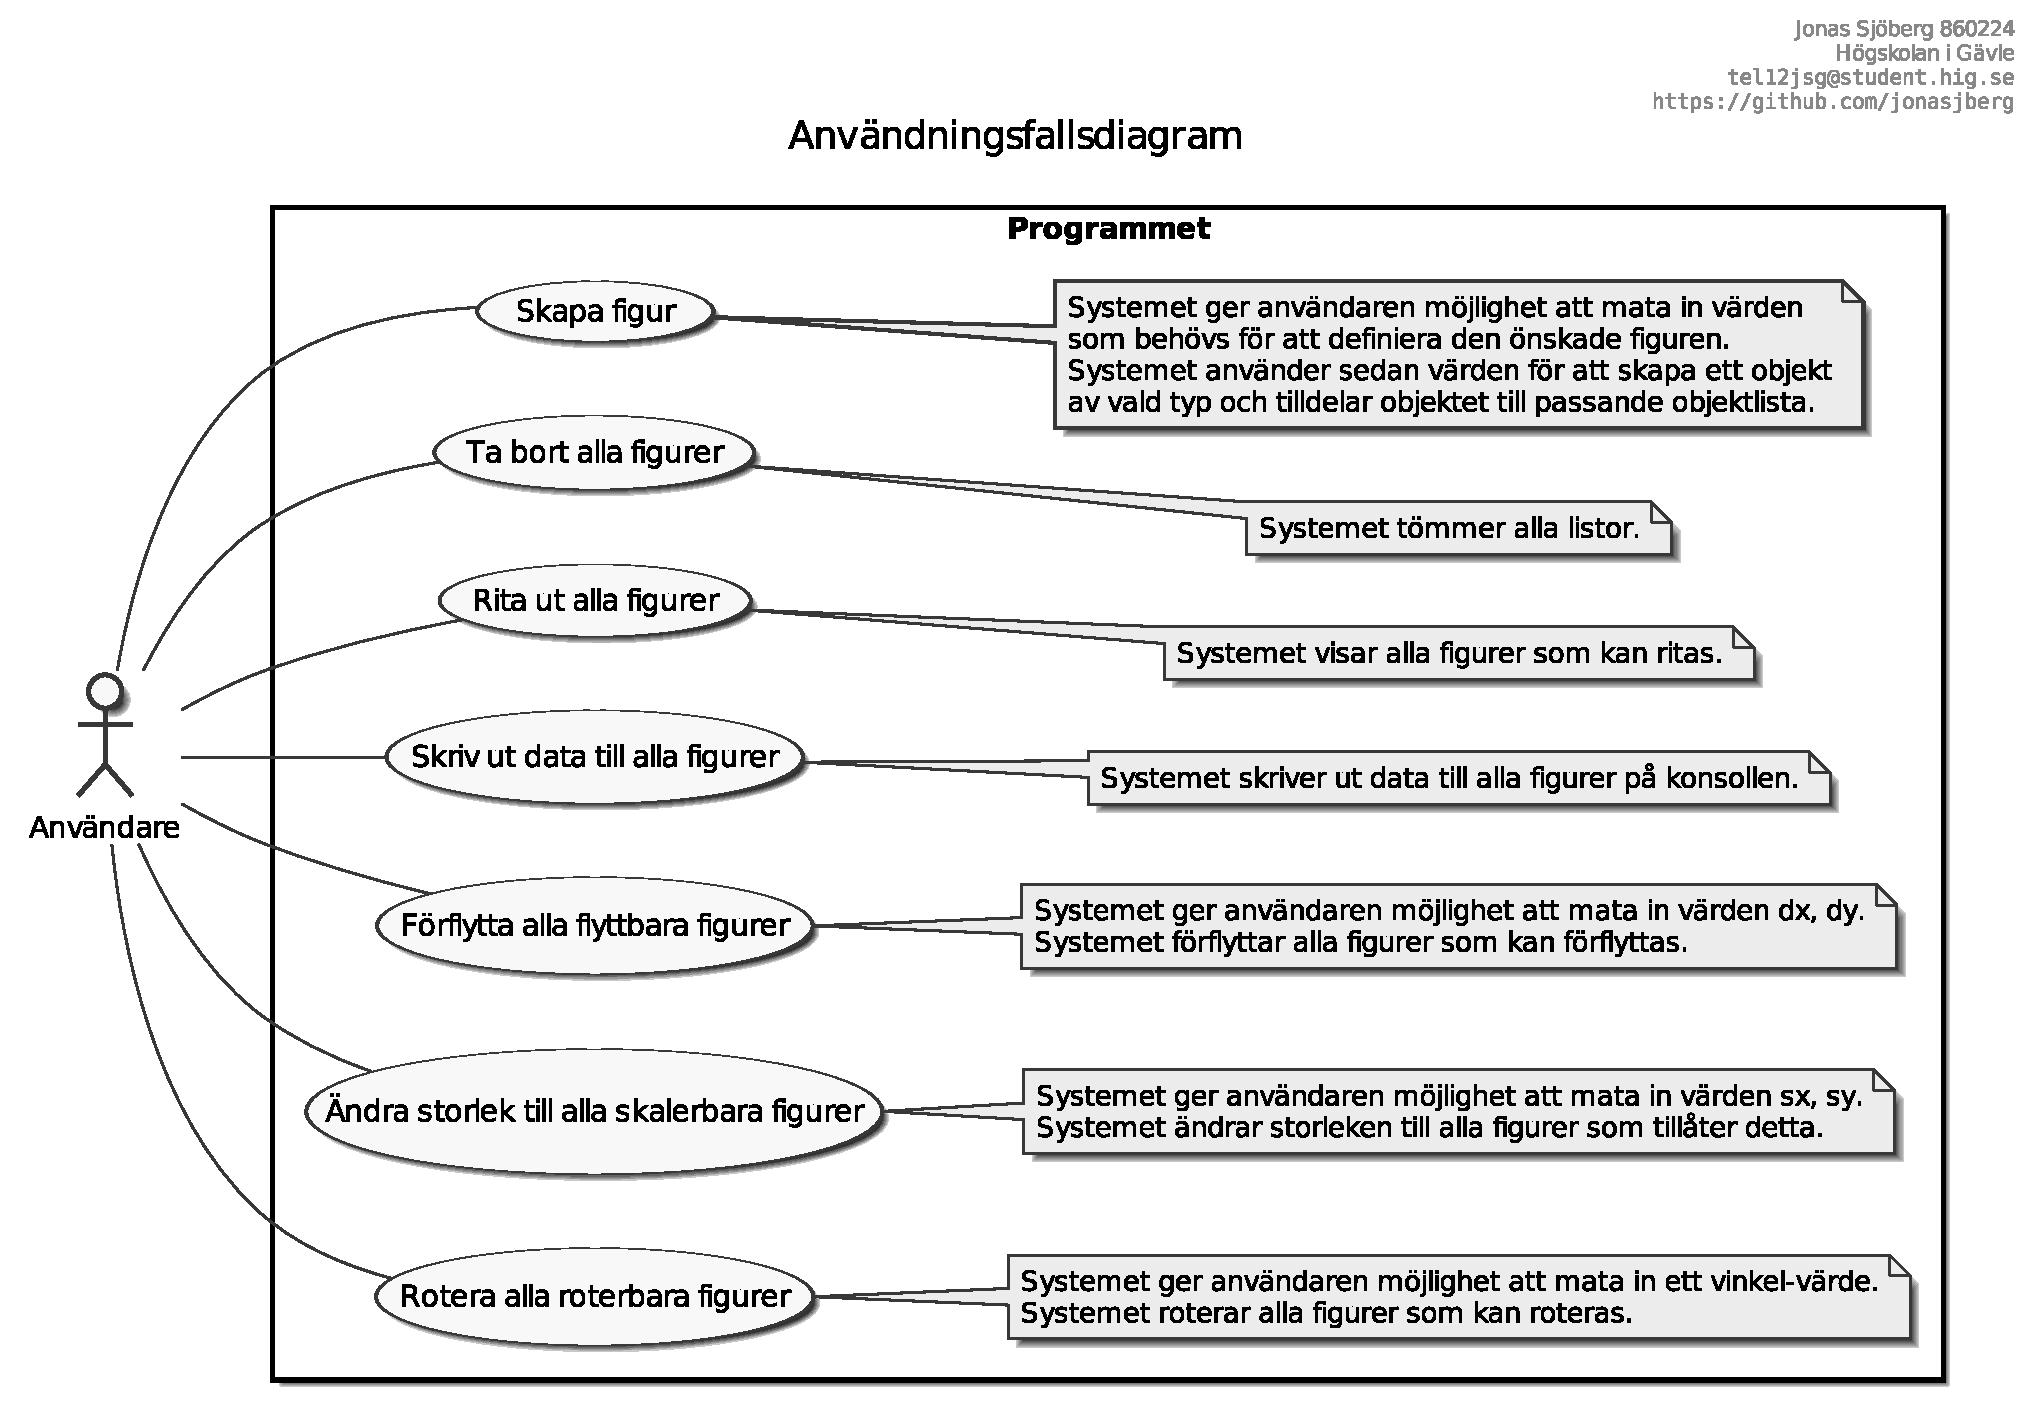
\includegraphics[width=\linewidth]{diagram/usecase.eps}
\caption{Användningsfallsdiagram (\texttt{diagram/usecase.eps})}
\label{fig:usecase}
\end{figure}

\subsection*{Arbetsmetod}
\addcontentsline{toc}{subsection}{Arbetsmetod}
\begin{itemize}
    \item Koden skrivs i utvecklingsmiljön \texttt{Intellij IDEA} under
    \texttt{Linux 3.19.0-28-generic} och kompileras samt exekveras med följande
    \texttt{Java}-version:
    \begin{verbatim}
    > $ java -version
    java version "1.7.0_79"
    OpenJDK Runtime Environment (IcedTea 2.5.6) (7u79-2.5.6-0ubuntu1.15.04.1)
    OpenJDK Server VM (build 24.79-b02, mixed mode)
    \end{verbatim}

    \item Rapporten skrivs i \latex med texteditorn \texttt{Vim} och kompileras
    till pdf med \texttt{latexmk}.
    \par Diagram och figurer skrivs i \texttt{PlantUML}-format och renderas med
    \texttt{Graphviz}. Resultatet förhandsgranskas i realtid med hjälp av
    plugins i \texttt{Intellij IDEA}.

    \item För revisionskontroll används \texttt{Git}.
\end{itemize}

UML-diagram och dokumentation uppdateras löpande parallellt med källkoden.
Förändringar i källkoden har kommit att följa uppdaterade diagram likväl som
diagrammen har behövt uppdateras för att reflektera förändrad källkod eller
funktionalitet.
\par Varje uppgift finns representerad som en separat utvecklingsgren
(\emph{branch}) i \texttt{Git}. På så vis kan varje uppgift utvecklas oberoende
utan redundans och filduplicering. Det är också mycket enkelt att propagera
förändringar mellan grenar och individuella \emph{commits} med hjälp av
ändamålsriktiga ``diff''-verktyg. Ett sådant ingår i standarddistributioner av
\texttt{Git}, ett annant exempel är \texttt{Meld}.


\subsection*{Källkod}
\addcontentsline{toc}{subsection}{Källor}
% TODO: Lägg till URL till specifikt repo ..
\par Källkod till programmet och rapporten finns att hämta på \url{https://github.com/jonasjberg}.
